\section{Question 5 (Theorectial) and 4 (Simulation)-Natural and Forced Response}

The total response of a circuit can be teased apart into a forced response plus a natural response. These responses can be combined using the principle of superposition. This principle pressupose the addition of the natural response and the forced response, both calculated in question 3 and 4.

\subsection{Theoretical Analysis}



\subsection{Simulation Analysis}
Once again, a transient analysis was made in order to meet the goal above. The main difference between the analysis in point 3 and this one is that Vs was considered a sinusoidal voltage source. This way, the plot obtained is the sum of both responses.

\begin{figure}[ht] \centering
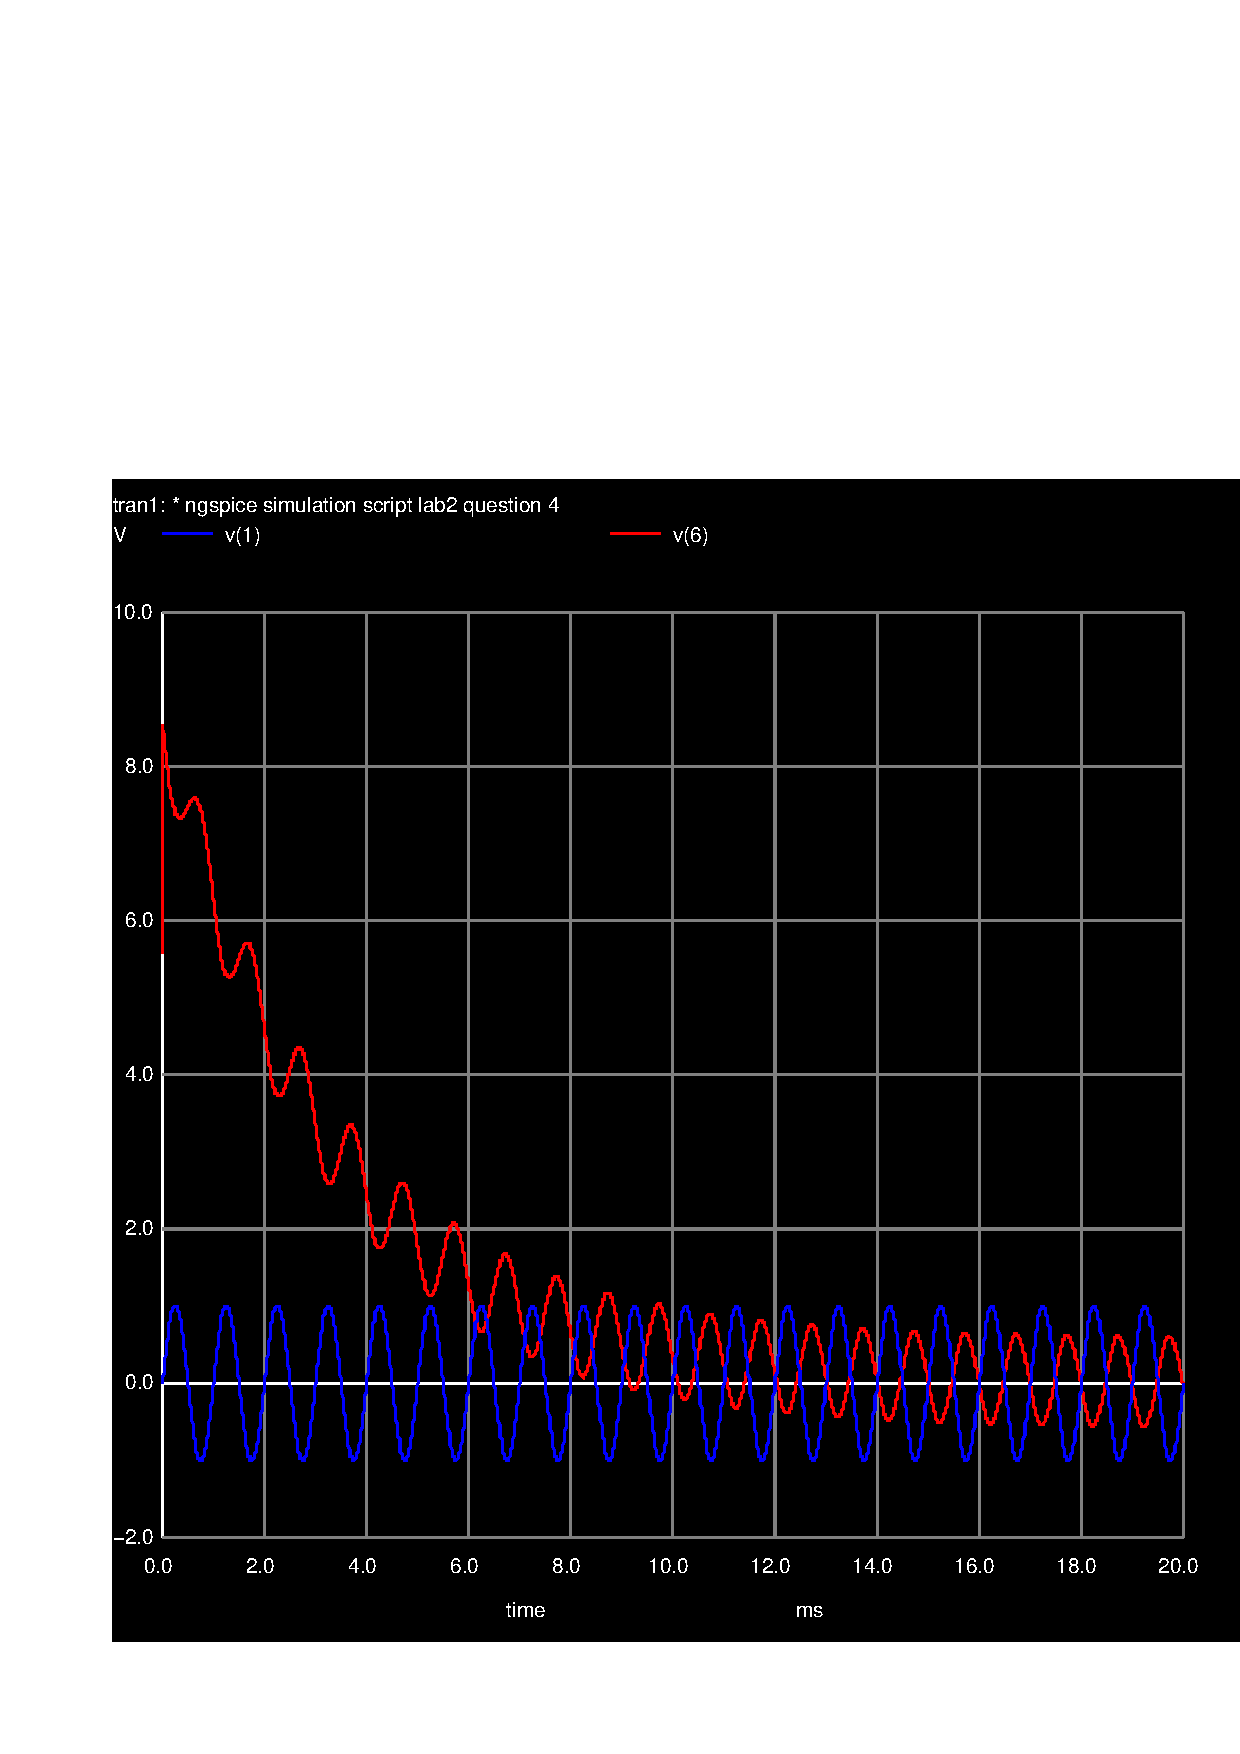
\includegraphics[width=0.9\linewidth]{sim4.pdf}
\caption{Circuit analysed.}
\label{fig:sim4}
\end{figure}

